\documentclass[10.5pt]{article}
\usepackage{xeCJK}%preamble part
\usepackage{graphicx}
\usepackage{indentfirst}
\usepackage[a4paper, inner=1.5cm, outer=3cm, top=2cm, bottom=3cm, bindingoffset=1cm]{geometry}
\usepackage{epstopdf}
\usepackage{array}
\usepackage{fontspec}
\usepackage{gensymb}
\usepackage[lofdepth,lotdepth]{subfig}
\setCJKmainfont[BoldFont={SimHei}]{SimSun}
\setCJKmonofont{SimSun}
\setmainfont{Times New Roman}
\newCJKfontfamily[hei]\heiti{SimHei}
\setlength{\extrarowheight}{4pt}
\begin{document}
\title{\textbf{\fontsize{15.75pt}{\baselineskip}{太阳能电池和燃料电池实验报告}}} % 15.75pt is 3 号 in chinese
\author{\fontsize{12pt}{\baselineskip}{数33 赵丰 2013012178}}
\maketitle
\section{\textbf{\fontsize{12pt}{\baselineskip}{引言}}}
太阳能电池是一种利用半导体材料的光学特性将光能转化为电能的器件,燃料电池是将燃料中的化学能直接转化为
电能而不经过热能这一中间环节的器件,它们是两种新型的绿色能源。
本次实验将研究太阳能电池和燃料电池的输出特性。
\section{\textbf{\fontsize{12pt}{\baselineskip}{实验原理}}}

太阳能电池的工作原理:常见的太阳能电池可看作一种pn结,它的工作原理主要是光生伏特效应。当光照射到该半导体材料时,在半导体材料内部会产生电协势,如果有回路就会产生光生电流。
无光照射时,太阳能电池的电流电压特性叫做暗特性,由肖克莱方程可以描述:
\begin{equation}
I=I_s [exp(\frac{eV}{k_0 T})-1]
\end{equation}
在有光照射时,光电流$I_L$一部分流经正偏的pn结,另一部分为输出电流$I$,其大小为:
\begin{equation}
I=I_L-I_S [exp(\frac{eV}{k_0 T})-1]
\end{equation}
有两种极端情况是在太阳能电池的光特性分析中必须考虑的,其一是负载电阻$R_L=0$,此时光电池的输出电流称之为闭路电流$I_{SC}$.
其二是负载电阻$RL \rightarrow \infty $,此时光电池两端的电压称之为开路电压$V_{oc}$.
太阳能电池的转换效率$\eta$定义为输出电能$P_{out}$与入射光能$P_{in}$的比值,在入射光强一定的情况下,极大化$P_{out}=I_{out} U_{out}$可提高
效率。$P_{out}$的最大值相当于在光电池的$I-V$特性曲线上的找到坐标乘积最大的点,此时$I_m V_m$构成一个最大功率矩形。

燃料电池工作原理:
氢氧燃料电池发生的总的化学反应为:
\begin{equation}
2H_2 + O_2 ==2H_2 O
\end{equation}

\begin{equation}
\rho=\frac{E_{max}}{E_{min}}
\end{equation}

\section{\textbf{\fontsize{12pt}{\baselineskip}{结果与讨论}}}
\subsection{\textbf{\fontsize{12pt}{\baselineskip}{计算的数据、结果}}}


1.太阳能电池暗特性测试
变压范围为-30V~30V,测得的I-V特性曲线以及用式(1)拟合的结果如下图Figure 1 所示:
\begin{figure}[!ht]
\centering
\caption{太阳能电池无光照条件下的伏安特性曲线}
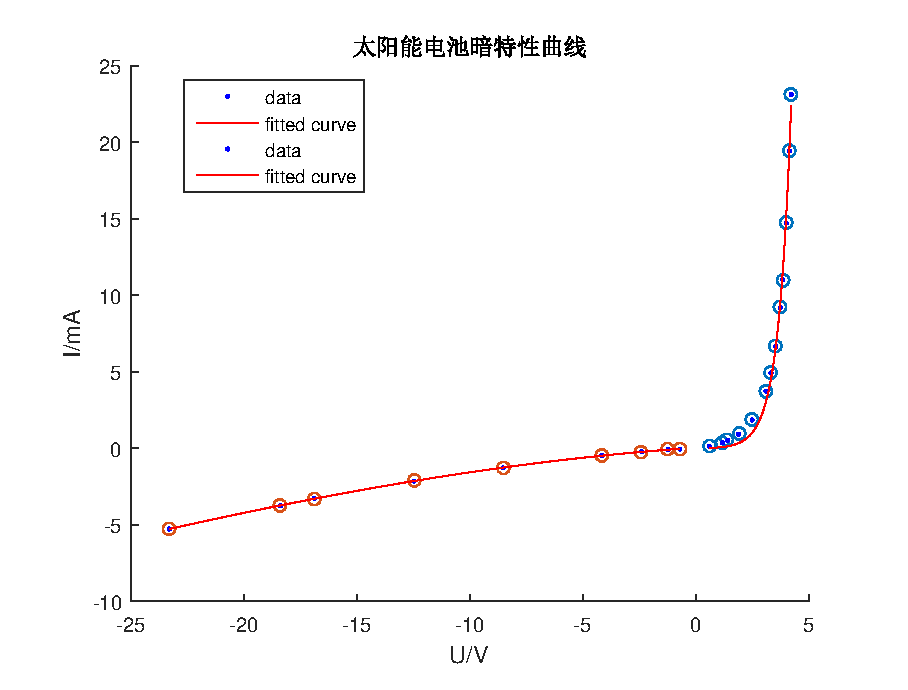
\includegraphics[width=400pt]{DimCharacteristic.eps}
\end{figure}

2 太阳能电池光照特性测试

1) 不加滤色片、在两种不同光强条件下光电池的$I-V$特性曲线如下图Figure 2所示:
\begin{figure}[!ht]
\centering
\caption{两种不同光强条件下光电池的$I-V$特性曲线}
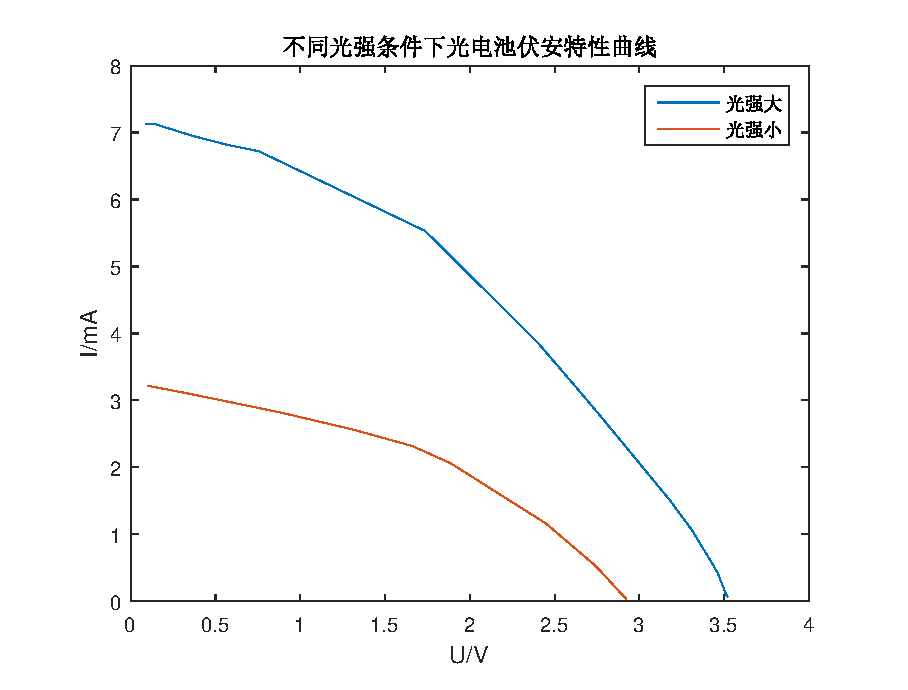
\includegraphics[width=350pt]{CurrentVoltageCurve.eps}
\end{figure}
由上图可估计出两种光强条件下的输出参数,其中$P_m$由曲线拟合算出:
\newpage

\begin{table}[!ht]
\centering
\begin{tabular}{ccccc}
\hline
&$I_{sc}(mA)$&$U_{oc}(V)$&$P_m(mW)$&占空系数(\%)\\
\hline
光强大&7.1&3.5&9.8&39\\
光强小&3.2&2.9&3.9&42\\
\hline
\end{tabular}
\caption{两种光强条件下光电池的输出参数}
\end{table}

可以看出,随光强的增大,光电池的$I_{sc}$和 $U_{oc}$都会增大,但$I_{sc}$增大得更快。
以较大的光强为例,下图Figure 3给出了输出功率$P$随$U$变化的曲线:
\begin{figure}[!ht]
\centering
\caption{光电池的输出电流和输出功率随电压变化曲线}
\includegraphics[width=400pt]{OutputSolarCellCurve.pdf}
\end{figure}
2)在最大光强条件下,加载波长分别为546nm和577nm的滤光片,测量光电池的I-V特性,汇总数据如下图Figure 4所示:
\begin{figure}[!ht]
\centering
\caption{不同单色光照条件下燃料电池的I-V关系}
\includegraphics[width=400pt]{DifferentWaveLengthSolarCellOutput.pdf}
\end{figure}
由上图可见,相同电压下输出功率随波长增大而增大。
\newline

3)使用加热器对光电池加热到45度左右,再次测量该温度范围下燃料电池的I-V关系,与常温下的实验数据进行对比,汇总数据如下图所示:
\begin{figure}[!ht]
\centering
\caption{不同温度条件下燃料电池的I-V关系}
\includegraphics[width=400pt]{DifferentTemperatureSolarCellOutput.pdf}
\end{figure}


3.质子交换膜电解池的特性测量
根据Faraday 电解定律,在标准状况下电解水时产生氢气的产生量为$V_{H_2}=\frac{It}{2F}\times 22.4$,其中$F=e N_A$,为Faraday 常数,$V_{H_2}$单位为升。
若实验时的摄氏温度为T,则由理想气体状态方程,氢气的产生量应为:
\begin{equation}
V_{H_2}=\frac{273.15+T}{273.15} \frac{It}{2F} \times 22.4
\end{equation}
实验室的温度为$T=26.5 \degree C$,于是可求得
$V_{H_2}=0.127 \times It$,I为输入电流,t为电解时间。
根据对I和t的测量结果,由上式可计算氢气的理论产生量,与实测结果对比,整理为如下形式的表格:
\begin{table}
\centering
\begin{tabular}{ccccc}
\hline
输入电流 I(A)&输入电压U(V)&测量时间t& $H_2$ 产生量$(V(({cm}_3))$&$H_2$产生量理论值$(V(({cm}_3))$\\
\hline
0.1&2&7分49s&5&5.96\\
0.2&2.12&5分56s&8&9.04\\
0.3&2.20&5分44s&12&13.1\\
\hline
\end{tabular}
\caption{电解池特性测量表}
\end{table}

实验中还测定了在$I=0.3A$时的氧气产生量,计时时间与氢气相同,$V_{O_2}=6 {cm}_3$,为氢气产生量的一半,理论结果为$6.55 {cm}_3$.


4.燃料电池输出特性测量
固定电解电流为297mA左右, 通过调节负载电阻,可得到燃料电池的输出电压与输出电流的关系如下图所示:
\begin{figure}[!ht]
\centering
\caption{燃料电池的输出电压与输出电流的关系}
\includegraphics[width=400pt]{figure_1.pdf}
\end{figure}
\newline

计算可得该燃料电池的最大输出功率为120.96mW,
以理想电动势为1.48V代入计算,可得最大输出功率下对应的效率为27.5\%




\subsection{\textbf{\fontsize{12pt}{\baselineskip}{讨论分析}}}

\section{\textbf{\fontsize{12pt}{\baselineskip}{结论}}}

通过本次实验,得出以下结论:
\begin{enumerate}
\item 太阳能电池和燃料电池的效率不超过40\%,和一般化学电池相比,效率偏低,还不适合大规模使用。
\item 保证太阳能电池和燃料电池正常工作需要有稳定的光源或燃料供应,否则输出电压不稳。
\item 太阳能电池和燃料电池输出特性受负载影响较大。
\end{enumerate}

\end{document}